\begin{flushright} {\tiny {\color{gray} python\_codes/fieldstone\_125/text.tex}} \end{flushright}

%\lstinputlisting[language=bash,basicstyle=\small]{python_codes/fieldstone_125/keywords}

\begin{center}

\fbox{\textbf{\huge \color{teal} P}}
Code at \url{https://github.com/cedrict/fieldstone/tree/master/python_codes/fieldstone_125}
\end{center}

\par\noindent\rule{\textwidth}{0.4pt}

%--------------------------------------------------------------------------------------------


To quote Wikipedia\footnote{\url{https://en.wikipedia.org/wiki/Voronoi_diagram}}:
``In mathematics, a Voronoi diagram is a partition of a plane into regions close to each of a given set of objects. 
In the simplest case, these objects are just finitely many points in the plane (called seeds, sites, or generators). 
For each seed there is a corresponding region, called a Voronoi cell, consisting of all points of the plane closer to 
that seed than to any other. The Voronoi diagram of a set of points is dual to its Delaunay triangulation. ''

%-----------------------------
\subsubsection*{Test \# 1}

\begin{center}
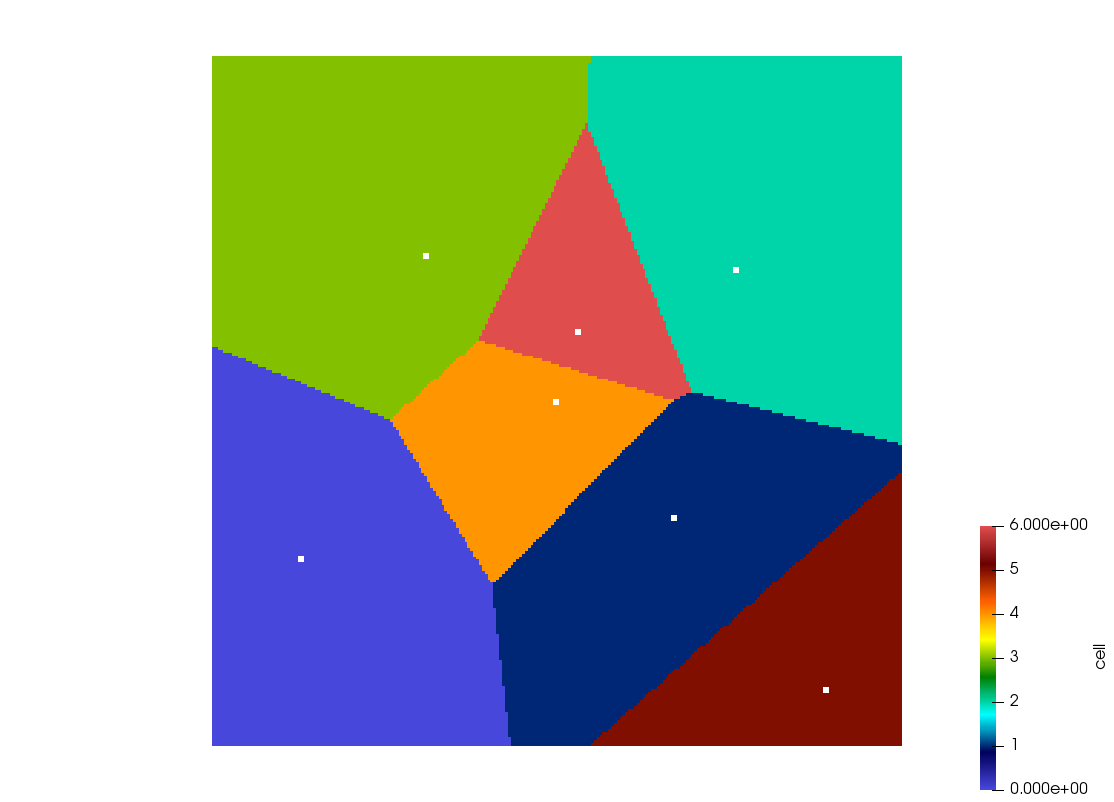
\includegraphics[width=6cm]{python_codes/fieldstone_125/results/diagram.png}\\
{\captionfont Example with 7 seeds.}
\end{center}


%-----------------------------
\subsubsection*{Test \# 2}

\begin{center}

\includegraphics[width=6cm]{python_codes/fieldstone_125/results/test2_a}

\includegraphics[width=6cm]{python_codes/fieldstone_125/results/test2_b}\\
{\captionfont Examples with 27 random seeds.}
\end{center}

%-----------------------------
\subsubsection*{Test \# 3}

\begin{center}

\includegraphics[width=6cm]{python_codes/fieldstone_125/results/test3}\\
{\captionfont Examples with 111 random seeds. Approx 310s.}
\end{center}



